\documentclass[DIV=calc]{scrartcl}
\usepackage[utf8]{inputenc}
\usepackage[T1]{fontenc}
\usepackage[ngerman]{babel}
\usepackage{graphicx}
\usepackage[draft, markup=underlined]{changes}
\usepackage{csquotes}
\usepackage{eurosym}
\usepackage{pdfpages}
\usepackage{ulem}
%\usepackage[dvipsnames]{xcolor}
\usepackage{paralist}
\usepackage{fixltx2e}
%\usepackage{ellipsis}
\usepackage[tracking=true]{microtype}

\usepackage{lmodern}              % Ersatz fuer Computer Modern-Schriften
%\usepackage{hfoldsty}

%\usepackage{fourier}             % Schriftart
\usepackage[scaled=0.81]{helvet}     % Schriftart

\usepackage[hyphens]{url}
%\usepackage{tocloft}             % Paket für Table of Contents

\usepackage{xcolor}
\definecolor{urlred}{HTML}{660000}

\usepackage{hyperref}
\hypersetup{colorlinks=false}

%\usepackage{mdwlist}     % Änderung der Zeilenabstände bei itemize und enumerate
% \usepackage{draftwatermark} % Wasserzeichen ``Entwurf''
% \SetWatermarkText{Antrag}

\parindent 0pt                 % Absatzeinrücken verhindern
\parskip 12pt                 % Absätze durch Lücke trennen

\setlength{\textheight}{23cm}
\usepackage{fancyhdr}
\pagestyle{fancy}
\fancyhead{} % clear all header fields
\cfoot{}
\lfoot{Zusammenkunft aller Physik-Fachschaften}
\rfoot{www.zapfev.de\\stapf@zapf.in}
\renewcommand{\headrulewidth}{0pt}
\renewcommand{\footrulewidth}{0.1pt}
\newcommand{\gen}{*innen}
\addto{\captionsngerman}{\renewcommand{\refname}{Quellen}}

%%%% Mit-TeXen Kommandoset
\usepackage[normalem]{ulem}
\usepackage{xcolor}
\usepackage{xspace} 

\newcommand{\replace}[2]{
    \sout{\textcolor{blue}{#1}}~\textcolor{blue}{#2}}
\newcommand{\delete}[1]{
    \sout{\textcolor{red}{#1}}}
\newcommand{\add}[1]{
    \textcolor{blue}{#1}}

\newif\ifcomments
\commentsfalse
%\commentstrue

\newcommand{\red}[1]{{\ifcomments\color{red} {#1}\else{#1}\fi}\xspace}
\newcommand{\blue}[1]{{\ifcomments\color{blue} {#1}\else{#1}\fi}\xspace}
\newcommand{\green}[1]{{\ifcomments\color{green} {#1}\else{#1}\fi}\xspace}

\newcommand{\repl}[2]{{\ifcomments{\color{red} \sout{#1}}{\color{blue} {\xspace #2}}\else{#2}\fi}}
%\newcommand{\repl}[2]{{\color{red} \sout{#1}\xspace{\color{blue} {#2}}\else{#2}\fi}\xspace}

\newcommand{\initcomment}[2]{%
	\expandafter\newcommand\csname#1\endcsname{%
		\def\thiscommentname{#1}%
		\definecolor{col}{rgb}{#2}%
		\def\thiscommentcolor{col}%
}}

% initcomment Name RGB-color
\initcomment{Philipp}{0, 0.5, 0}

%\renewcommand{\comment}[1]{{\ifcomments{\color{red} {#1}}{}\fi}\xspace}

\renewcommand{\comment}[2][\nobody]{
	\ifdefined#1
	{\ifcomments{#1 \expandafter\color{\thiscommentcolor}{\thiscommentname: #2}}{}\fi}\xspace
	\else
	{\ifcomments{\color{red} {#2}}{}\fi}\xspace
	\fi
}

\newcommand{\zapf}{ZaPF\xspace}

\let\oldgrqq=\grqq
\def\grqq{\oldgrqq\xspace}

\setlength{\parskip}{.6em}
\setlength{\parindent}{0mm}

%\usepackage{geometry}
%\geometry{left=2.5cm, right=2.5cm, top=2.5cm, bottom=3.5cm}

% \renewcommand{\familydefault}{\sfdefault}




\begin{document}

\hspace{0.87\textwidth}
\begin{minipage}{120pt}
	\vspace{-1.8cm}
	
\includegraphics[width=80pt]{../logo.pdf}
	\centering
	\small Zusammenkunft aller Physik-Fachschaften
\end{minipage}

\begin{center}
  \huge{Positionspapier: Unterzeichnung der Studiumsqualitätsverordnung}\vspace{.25\baselineskip}\\
  \normalsize
\end{center}
\vspace{1cm}

%%%% Metadaten %%%%

% \paragraph{Addressierte:} - HRK- Uni Präsidenten- CCC im CC- FZS (interdisziplinäre Reso) - DPG im CC- DFN -Metafa -Landesastenkonferenzen -Deutschen Initiative fuer Netzwerkinformation (DINI) 
 

% \paragraph{Antragstellende:} Jörg (Siegen), Tobi (Düsseldorf), ChrisPi (Heidelberg), Jörg (Alumni)

%%%% Text des Antrages zur veröffentlichung %%%%

% \section*{Antragstext}

Die ZaPF unterzeichnet die angehängte Resolution zur Änderung der Studiumsqualitätsverordnung in NRW.


\vspace{1cm} 

\vfill
\begin{flushright}
	Verabschiedet am 23. Mai 2021 \\
	auf der Digital-ZaPF hosted in Rostock.
\end{flushright}

\includepdf[pages={2,3}]{Reso.pdf}

\end{document}
